%%%%%%%%%%%%%%%%%%%%%%%%%%%%%%%%%%%%%%%%%%%%%%%%%%%%%%%%%%
% # Appendix: C-Test Results
%%%%%%%%%%%%%%%%%%%%%%%%%%%%%%%%%%%%%%%%%%%%%%%%%%%%%%%%%%

\chapter{C-test results}\label{app-results-ctest}

% ORC and SRC Figures
% \begin{figure}
% \caption{English C-test proficiency scores in the ORC and SRC studies (Max = 50)} \label{fig:app-ctest}
% \raggedright\setstretch{1}
% 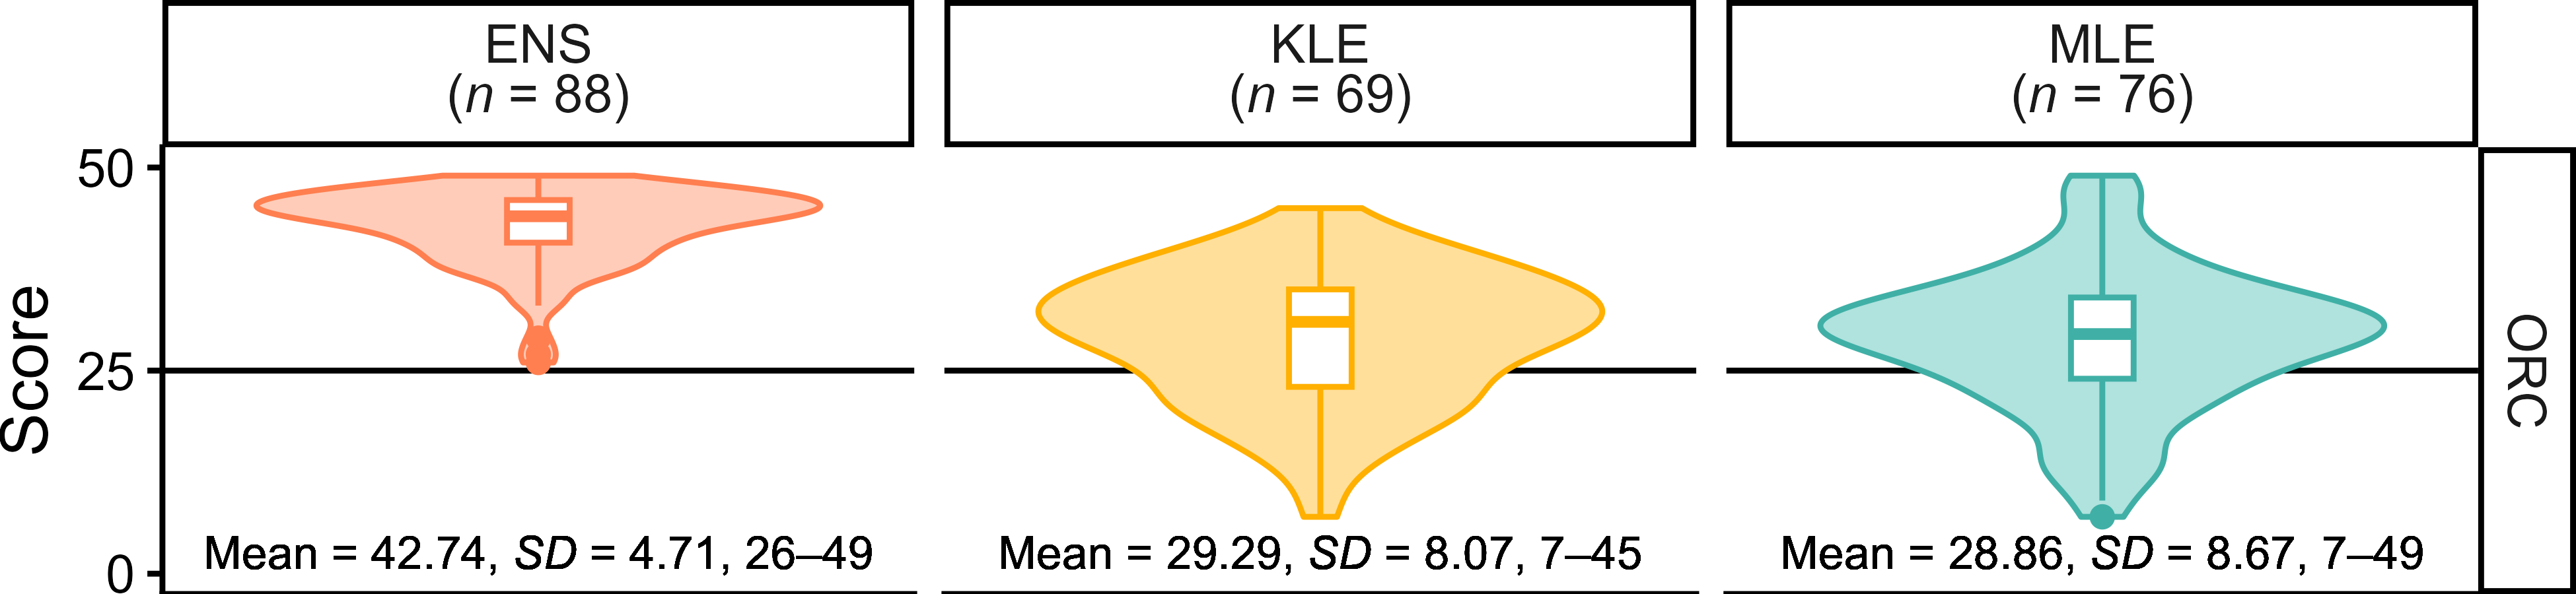
\includegraphics{../analysis/plots/orc_ctest.png}
% 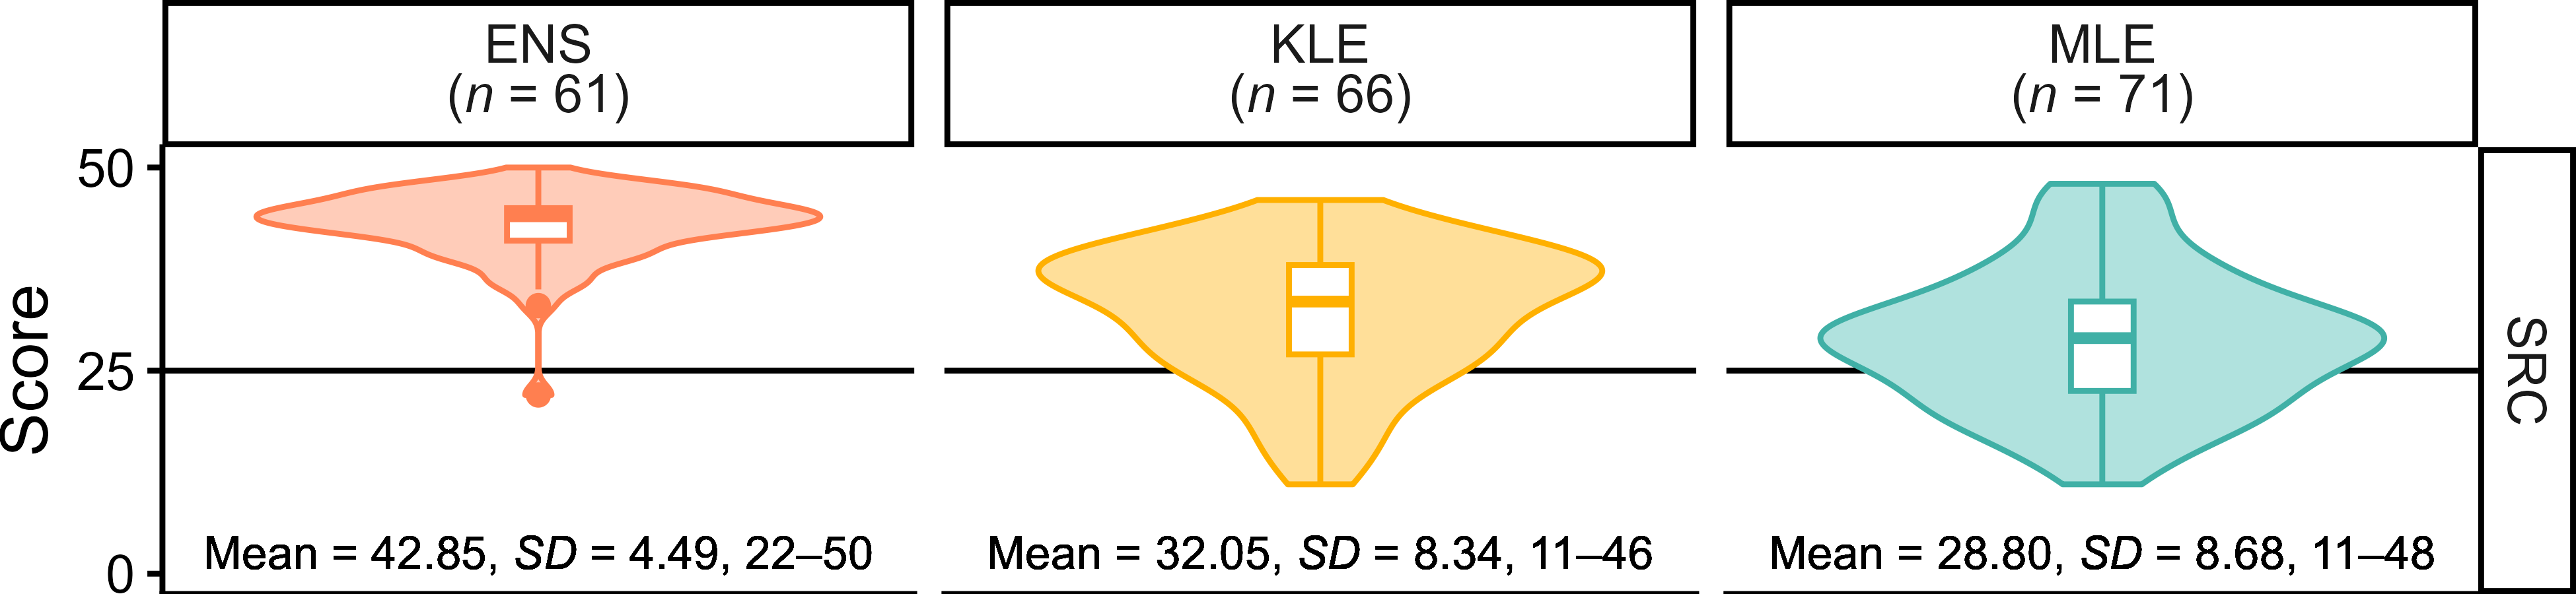
\includegraphics{../analysis/plots/src_ctest.png}
% \textit{Note}. Horizontal line represents 50\% accuracy; center lines in boxplots are medians, boxes are interquartile ranges, and whiskers extend to data points within 1.5 times the interquartile range.
% \vspace{-12pt}
% \end{figure}

% ORC Model
\begin{table}
\caption{Summary of mixed-effects logistic regression model on C-test accuracy in the ORC study}\label{tab:app-orc-ctest-accuracy-model}
\raggedright\setstretch{1}
\begin{tabu} to \textwidth {X[l]X[r]X[r]X[r]X[r]}\toprule
Parameter & Estimate~($\hat{\beta}$) & \textit{SE} & $z$ & $p$ \\\midrule
\csvreader[late after line=\\,late after last line=\\\bottomrule]
{../analysis/tables/orc_ctest_accuracy_model.csv}{}{\csvcoli & \csvcolii & \csvcoliii & \csvcoliv & \csvcolv}
\end{tabu}
\newline\textit{Note}. Model formula: Accuracy \~{} Group + (1 | Participant) + (1 + Group | Item); reference level:
ENS; estimate unit: logit; intercept: grand mean.
\vspace{-12pt}
\end{table}

% ORC Posthoc
\begin{table}
\caption{Post-hoc tests for C-test accuracy in the ORC study}\label{tab:app-orc-ctest-accuracy-posthoc}
\raggedright\setstretch{1}
\begin{tabu} to \textwidth {X[l]X[r]X[r]X[r]X[r]}\toprule
Contrast & Estimate~($\hat{\beta}$) & \textit{SE} & $z$ & $p$ \\\midrule
\csvreader[late after line=\\,late after last line=\\\bottomrule]
{../analysis/tables/orc_ctest_accuracy_posthoc.csv}{}{\csvcoli & \csvcolii & \csvcoliii & \csvcoliv & \csvcolv}
\end{tabu}
\newline\textit{Note}. Adjustment to $p$-values done via multiple $t$ method for 3 tests.
\vspace{-12pt}
\end{table}

% SRC Model
\begin{table}
\caption{Summary of mixed-effects logistic regression model on C-test accuracy in the SRC study}\label{tab:app-src-ctest-accuracy-model}
\raggedright\setstretch{1}
\begin{tabu} to \textwidth {X[l]X[r]X[r]X[r]X[r]}\toprule
Parameter & Estimate~($\hat{\beta}$) & \textit{SE} & $z$ & $p$ \\\midrule
\csvreader[late after line=\\,late after last line=\\\bottomrule]
{../analysis/tables/src_ctest_accuracy_model.csv}{}{\csvcoli & \csvcolii & \csvcoliii & \csvcoliv & \csvcolv}
\end{tabu}
\newline\textit{Note}. Model formula: Accuracy \~{} Group + (1 | Participant) + (1 + Group | Item); reference level:
ENS; estimate unit: logit; intercept: grand mean.
\vspace{-12pt}
\end{table}

% SRC Posthoc
\begin{table}
\caption{Post-hoc tests for C-test accuracy in the SRC study}\label{tab:app-src-ctest-accuracy-posthoc}
\raggedright\setstretch{1}
\begin{tabu} to \textwidth {X[l]X[r]X[r]X[r]X[r]}\toprule
Contrast & Estimate~($\hat{\beta}$) & \textit{SE} & $z$ & $p$ \\\midrule
\csvreader[late after line=\\,late after last line=\\\bottomrule]
{../analysis/tables/src_ctest_accuracy_posthoc.csv}{}{\csvcoli & \csvcolii & \csvcoliii & \csvcoliv & \csvcolv}
\end{tabu}
\newline\textit{Note}. Adjustment to $p$-values done via multiple $t$ method for 3 tests.
\vspace{-12pt}
\end{table}